\hypertarget{sweetn-low}{%
\section{Sweet'n Low}\label{sweetn-low}}

\begin{figure}[!ht]
  \begin{adjustwidth}{-\oddsidemargin-1in}{-\rightmargin}
    \centering
    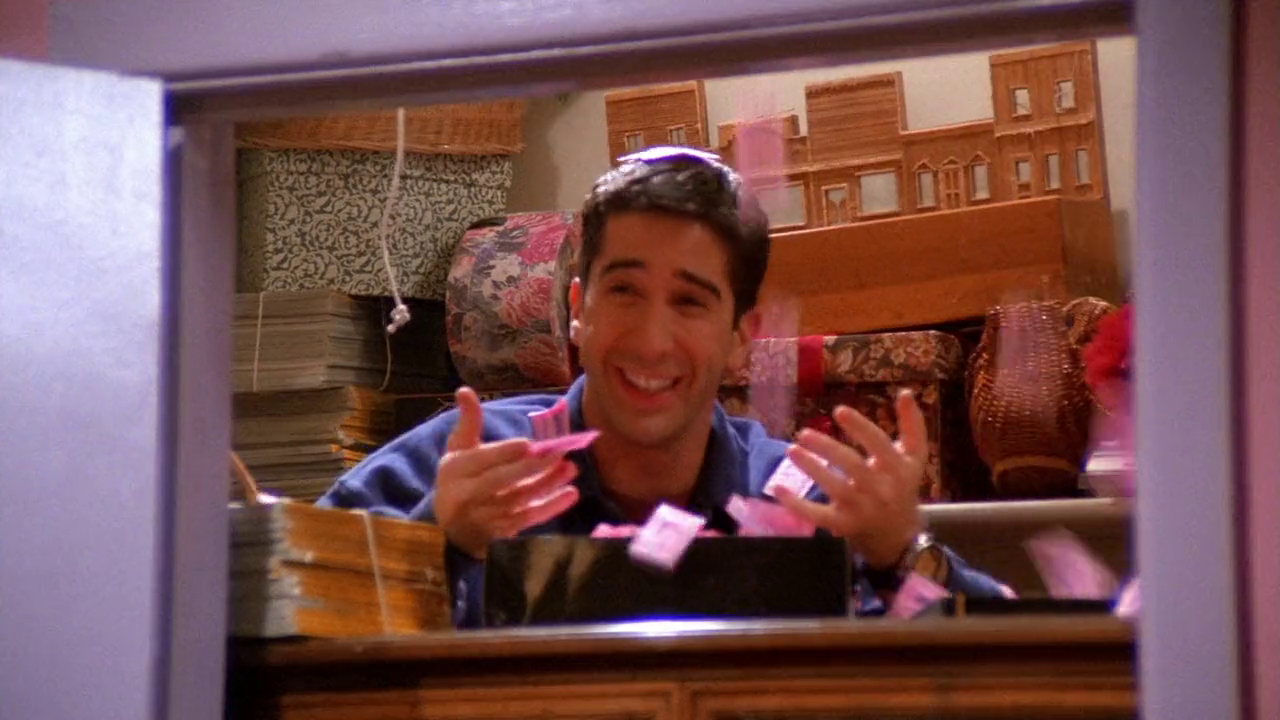
\includegraphics[trim={0 5cm 0 3cm,}, clip, width=\paperwidth]{./S01/img/8/sweet-n-low.png}
    % \caption{Sweet’n Low\label{fig:sweet-n-low}}
  \end{adjustwidth}
\end{figure}

Ross menciona que sua vó Althea adorava \emph{Sweet'n Low} (1957),
conhecida marca de adoçantes americana, que possui a característica
marcante do sachê cor de rosa.\footnote{\sloppy Sweet’n Low - Site oficial. \url{http://www.sweetnlow.com/brand}}

\hypertarget{brent-musburger}{%
\section{Brent Musburger}\label{brent-musburger}}

\begin{figure}[!ht]
  \begin{adjustwidth}{-\oddsidemargin-1in}{-\rightmargin}
    \centering
    
\includegraphics[trim={0 11cm 0 2cm,}, clip, width=\paperwidth]{./S01/img/8/brent-musburger.png}
    % \caption{Brent Musburger\label{fig:brent-musburger}}
  \end{adjustwidth}
\end{figure}

\begin{tcolorbox}[enhanced,center upper,
    drop fuzzy shadow southeast, boxrule=0.3pt,
    lower separated=false, breakable,
    colframe=black!30!dialogoBorder,colback=white]
\begin{minipage}[c]{0.16\linewidth}
  \raisebox{\dimexpr-\height+\ht\strutbox\relax}{
    \centering 
\includegraphics[width=1.4cm]{./assets/img/joey.png}
  }
   & \centering \scriptsize{Joey}
\end{minipage}
\hfill
\begin{minipage}[c]{0.8\linewidth}
  \textbf{- What?}\\
  - Que foi?
\end{minipage}

\medskip
\begin{minipage}[c]{0.16\linewidth}
  \raisebox{\dimexpr-\height+\ht\strutbox\relax}{
    \centering 
\includegraphics[width=1.4cm]{./assets/img/chandler.png}
  }
   & \centering \scriptsize{Chandler}
\end{minipage}
\hfill
\begin{minipage}[c]{0.8\linewidth}
  \textbf{- Nothing. Just your overcoat sounds remarkably like Brent Musburger.}\\
  - Nada. Seu casaco tem a voz de Brent Musburger.
\end{minipage}
\end{tcolorbox}

\saveparinfos
\noindent
\begin{minipage}[c]{0.5\textwidth}\useparinfo

Enquanto caminham para a recepção do enterro da vó de Ross e Monica,
Chandler menciona que o casaco de Joey soa como \emph{Brent Musburger}
(1939), narrador esportivo que iniciou sua carreira na \emph{CBS Sport}
em 1975. Na época do episódio estava na \emph{ABC/ESPN}, cobrindo
inclusive, como é visto, partidas de Futebol Americano.\footnote{\sloppy Brent Musburger Biography - VSIN. \url{https://www.vsin.com/about/brent-musburger-biography/}}

\end{minipage}\hfill
\begin{minipage}[c]{0.5\textwidth}

\begin{figure}
  \centering
  \begin{tikzpicture}
    \node [inner sep=0pt] at (0,0) {
      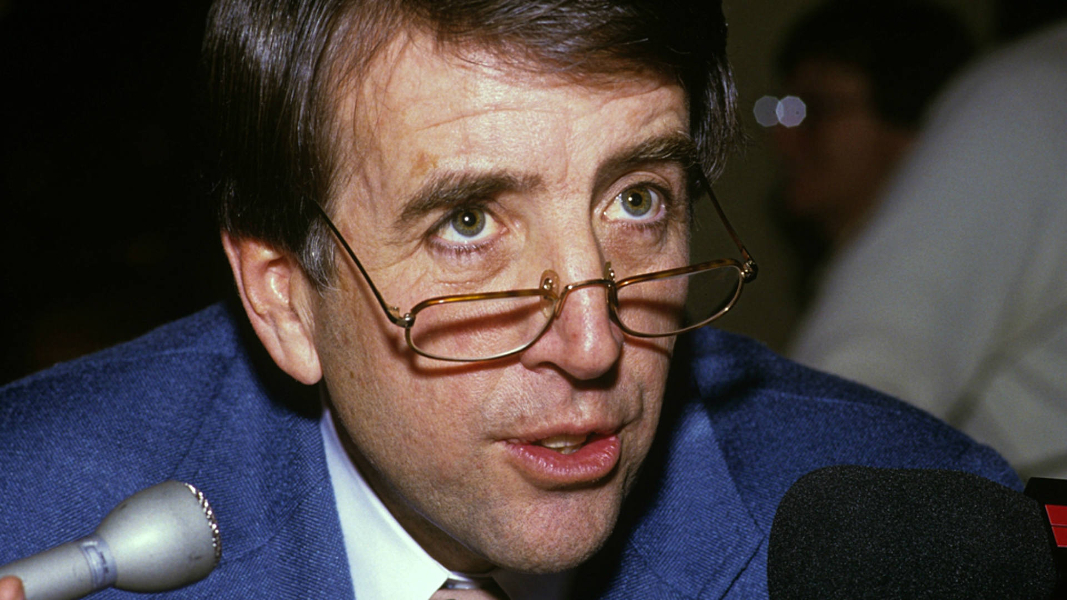
\includegraphics[width=0.8\textwidth,keepaspectratio]{./S01/img/8/brent-musburger-photo.jpg}
    };
    \draw [white, rounded corners=\ClipSep, line width=\ClipSep]
    (current bounding box.north west) --
    (current bounding box.north east) --
    (current bounding box.south east) --
    (current bounding box.south west) -- cycle
    ;
    \end{tikzpicture}
    \caption{Brent Musburger - Foto\label{fig:brent-musburger-foto}}
\end{figure}

\end{minipage}
